\paragraph{Architectuur}
Net zoals bij Bitcoin zijn de transacties de kern van de implementatie, waarbij er wederom gebruik wordt gemaakt van het \gls{UTXO} zoals beschreven bij de architectuur van Bitcoin. 
De architectuur van het Cardano netwerk bestaat uit drie soorten \glspl{node} die fundamenteel zijn voor de werking van het protocol: \textit{core}, \textit{relay} en \textit{edge} \glspl{node}.\textit{Core \glspl{node}} zijn de kern van het netwerk. Het zijn de enige \glspl{node} die geselecteerd kunnen worden om \gls{slot_leader} te worden, waardoor het de enige \glspl{node} zijn die een block kunnen creëren.
\textit{Relay \glspl{node}} worden gezien als de proxy tussen core \glspl{node} en het internet. Ze hebben geen stake in het netwerk, waardoor ze makkelijk te verplaatsten of veranderd kunnen worden.
\textit{Edge \glspl{node}} zijn de simpele \glspl{node} die iedereen kan uitvoeren. Deze \glspl{node} kunnen transacties aanmaken binnen het netwerk en aanbieden aan \textit{core} \glspl{node} via de \textit{relay} \glspl{node} \citep[Topology]{cardano_wiki}.

\paragraph{Discovery protocol}
\begin{wrapfigure}{r}{0.6\textwidth}
  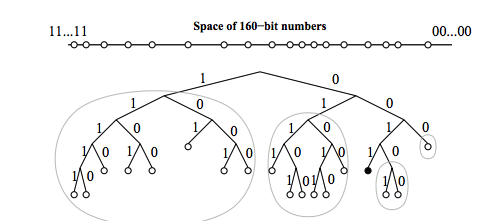
\includegraphics[width=0.6\textwidth]{kademlia}
  \caption{Binary Tree zoals in gebruik bij het Kademlia protocol, \cite{maymounkov2002kademlia}.}
  \label{kademlia_binary_tree}
\end{wrapfigure}

Om het netwerk te betreden wordt er gebruik gemaakt van een bestaand protocol genaamd Kademlia, wat gebaseerd is op het gebruik van een \acrfull{DHT} architectuur. Elke node wordt behandeld als een tak in een Binary Tree waarbij de positie van een \gls{node} bepaald wordt door een unieke prefix van de identificatie code van een \gls{node}. In fig. \ref{kademlia_binary_tree} is de positie van een \gls{node} met de prefix 0011 te zien. Het protocol garandeert dat elke \gls{node} in verbinding staat met een andere \gls{node}. Met deze garantie kan elke \gls{node} een andere \gls{node} lokaliseren aan de hand van de identificatie code \citep[p.~2]{maymounkov2002kademlia}.

\subsubsection{Informatie propagatie}
Berichten worden verstuurd voor het uitwisselen van informatie tussen deelnemers. Hierbij zijn drie abstracte types gedefinieerd: \textit{inv}, \textit{req} en \textit{data}. Net zoals bij Bitcoin wordt de \textit{inv} message gebruikt om aan te geven dat er data beschikbaar is. Het \textit{req} bericht wordt vervolgens gebruikt om beschikbare data op te vragen. De data wordt vervolgens verstuurd via een \textit{data} message. Berichten die bijvoorbeeld een block versturen zijn nader gespecificeerde \textit{data} berichten. Op deze drie types zijn alle berichten in het netwerk gebaseerd, bijvoorbeeld is het \textit{MsgBlock} bericht, die block informatie uitwisselt, gebaseerd op een \textit{data} bericht \citep{cardano_wiki:csl_app_level}. Een bericht kan verstuurd worden naar drie verschillende mediums: het versturen van een bericht naar een \gls{node}, de buren, en het gehele netwerk. Naar welk medium het bericht wordt verstuurd is opgenomen in de header van een bericht.
